\documentclass[pdftex,dvipsnames]{dissertation}

%%% MY PACKAGES
\usepackage{blindtext} % provide \blindtext, \Blindtext
\usepackage{lipsum}
% \usepackage{libertine} % nice font
% % ==  mathematical fonts ==
% \usepackage{ccfonts}  % mathematical fonts
% \usepackage[T1]{fontenc}  % mathematical fonts
% \renewcommand{\rmdefault}{cmr}% cmr = Computer Modern Roman
% % ==  mathematical fonts ==

%%% TOC per CHAPTER %%%
\usepackage{minitoc}

%%% SETUP TODO NOTES
% dep
\usepackage{xargs}   % Use more than one optional parameter in a new commands
\usepackage{xcolor}  % Coloured text etc.
% pkg
\usepackage[colorinlistoftodos,prependcaption,textsize=small,shadow]{todonotes}
% my alias
\newcommand{\itodo}[1]{\todo[inline]{#1}\PackageWarning{TODO ::}{#1}}
\newcommand{\miss}[1]{\todo[inline,backgroundcolor=white,bordercolor=black]{#1}\PackageWarning{TODO ::}{#1}}
\newcommandx{\unsure}[2][1=]{\todo[linecolor=red,backgroundcolor=red!25,bordercolor=red,#1]{#2}\PackageWarning{TODO ::}{#2!}}
\newcommandx{\change}[2][1=]{\todo[linecolor=blue,backgroundcolor=blue!25,bordercolor=blue,#1]{#2}\PackageWarning{TODO ::}{#2!}}
\newcommandx{\info}[2][1=]{\todo[linecolor=OliveGreen,backgroundcolor=OliveGreen!25,bordercolor=OliveGreen,#1]{#2}\PackageWarning{TODO ::}{#2!}}
\newcommandx{\plus}[2][1=]{\todo[linecolor=Plum,backgroundcolor=Plum!25,bordercolor=Plum,#1]{#2}\PackageWarning{TODO ::}{#2!}}

%%% DEFAULT PACKAGE
\usepackage{amsmath,mathtools,empheq}
\usepackage{amsthm}

%%% THEOREMS and ENVIROMENTS
\usepackage{thmtools}
\usepackage{thm-restate}
\declaretheorem[%
    name=Rationale,
    refname={Rationale,Rationales},
    Refname={Rationale,Rationales}
]{rationale}
\declaretheorem[%
    name={Security Claim},
    numbered={unless unique},
]{secclaim}

%%% OTHER PCKs FROM THE AUTHOR
\usepackage{longtable}
\usepackage{pdflscape}
\usepackage{enumitem}

%% COLORS %%
\definecolor{RoyalBlue}{cmyk}{1,0.5,0,0}
\definecolor{Black}{cmyk}{0,0,0,0}
\definecolor{alertred}{rgb}{0.80,0.12,0.12}
\definecolor{linkgreen}{RGB}{0,166,0}

%%% TOC STYLE : check in the dissertation class
% \setcounter{secnumdepth}{5}
% \setcounter{tocdepth}{5}
%

\newrobustcmd*{\fullfullcite}{%
    \AtNextCite{%
        \AtEachCitekey{%
            \defcounter{maxnames}{99}%
            \DeclareNameAlias{labelname}{given-family}%
        }%
    }%
    \fullcite
}

%% IMAGE AS SYMBOL

% % set the Bison QED symbol
% \renewcommand{\qed}{%
% \leavevmode\unskip\penalty9999 \hbox{}\nobreak\hfill%
% \quad\hbox{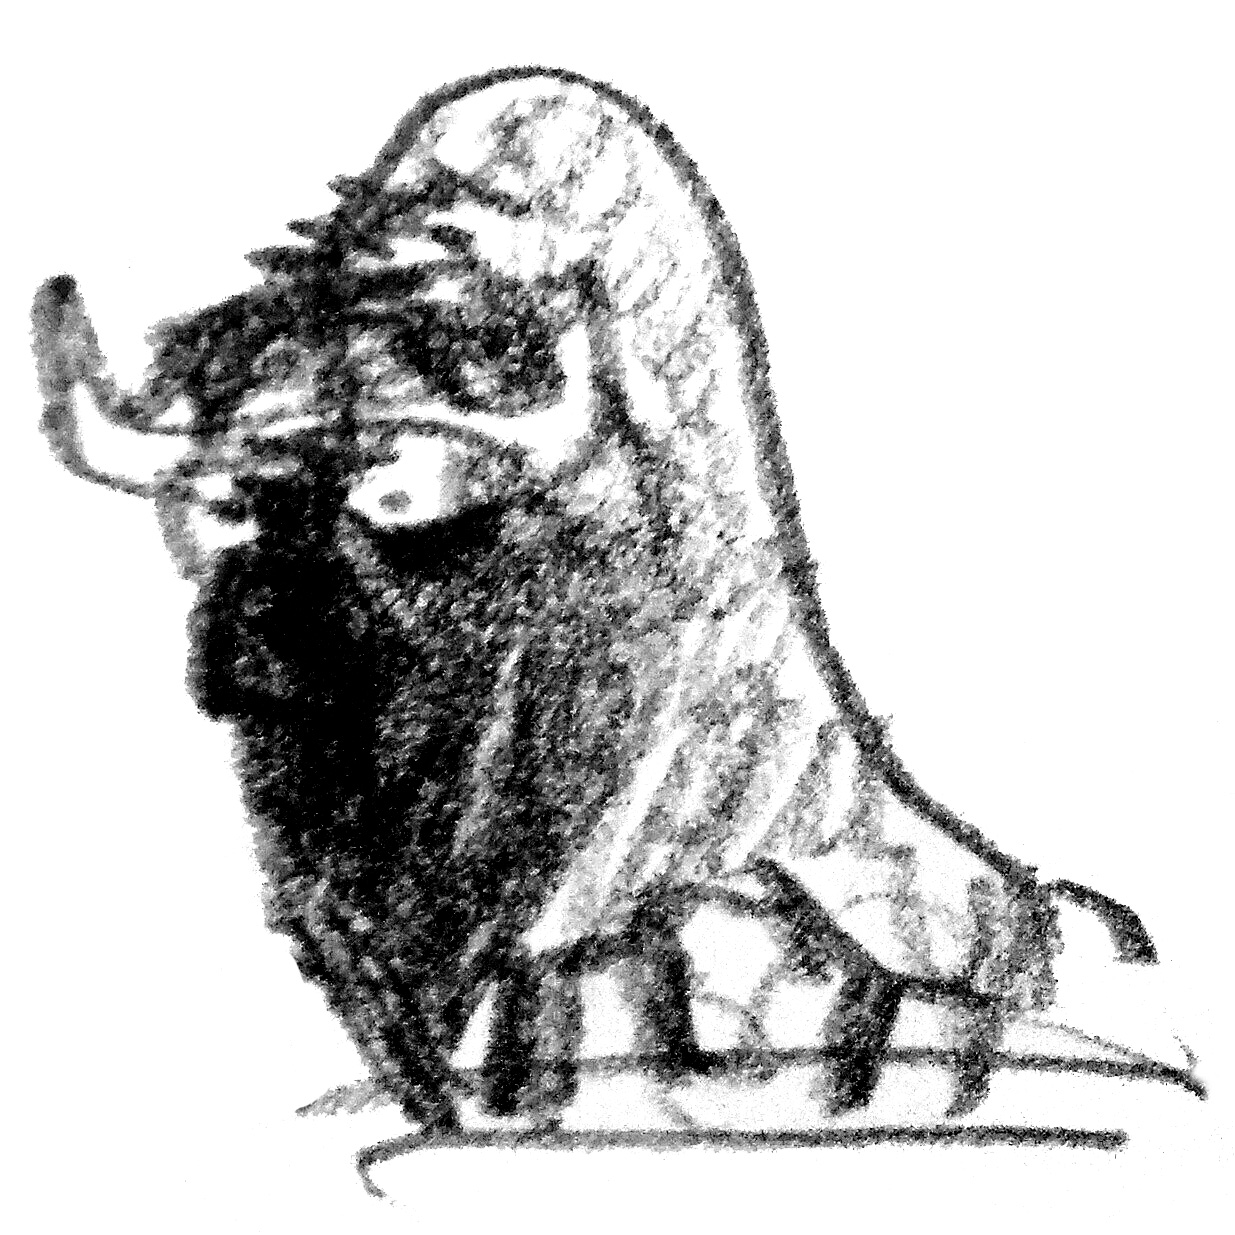
\includegraphics[height=1em]{bison/bison-qed.jpg}}}

\newcommand{\cpother}[1]{{\color{BlueGreen} #1}}
\newcommand{\cpmine}[1]{{\color{GreenYellow} #1}}

% --- my abbreviation ---------------------------------------------------------
\newcommand{\imgsrc}[1]{Image courtesy of #1}
\newcommand{\cfr}[1]{\Cf/ #1}

% --- math models -------------------------------------------------------------
\newcommand{\echoModelFreq}{\ensuremath{
    H_{ij}(f_k) = \sum_{\idxEch=0}^{\numEchs}
        \frac{\absCoeff_{ij}^r}{4 \pi \speedOfSound \tau_{ij}^r}
        \cste^{- \csti 2 \pi k \Fs \tau_{ij}^r / F}}}

\newcommand{\sumEcho}{\ensuremath{\sum_{\idxEch=0}^{\numEchs}}}
\newcommand{\echoModelTimeSimple}[1]{\ensuremath{\sumEcho \alpha_{#1}^{(r)} \delta(t - \tau_{#1}^{(r)})}}
\newcommand{\alltaus}[1]{\ensuremath{\{\tau_{#1}^{(r)}\}_{#1,r}}}
\newcommand{\allalphas}[1]{\ensuremath{\{\alpha_{#1}^{(r)}\}_{#1,r}}}

\newcommand{\icon}[1]{\raisebox{-.1\height}{\includegraphics[height=3ex]{#1}}}
\newcommand{\chaosIcon}{\icon{figures/blaster/chaos.png}}
% --- correct bad hyphenation
\hyphenation{op-tical net-works semi-conduc-tor}

% --- Algos and Methods names:
\newcommand{\mirage}{\textsc{Mirage}}
\newcommand{\separake}{\textsc{Separake}}
\newcommand{\brioche}{\textsc{Brioche}}
\newcommand{\blaster}{\textsc{Blaster}}
\newcommand{\blasterr}{\textsc{Blaster2}}
\newcommand{\lantern}{\textsc{Lantern}}
\newcommand{\dechorate}{d'\textsc{Echorate}}

%----------------
\usepackage{pgffor}
% for math stuff
\foreach \x in {a,...,z}{
  % mathbf
  \expandafter\xdef\csname bf\x \endcsname{\noexpand\ensuremath{\noexpand\mathbf{\x}}}
  % Bold symbol
  \expandafter\xdef\csname bs\x \endcsname{\noexpand\ensuremath{\noexpand\boldsymbol{\x}}}
  % Typewriter
  \expandafter\xdef\csname tt\x \endcsname{\noexpand\ensuremath{\noexpand\mathtt{\x}}}
}

\foreach \x in {A,...,Z}{
%   % Bold symbol -- bold
  \expandafter\xdef\csname bs\x \endcsname{\noexpand\ensuremath{\noexpand\boldsymbol{\x}}}
%   % mathbf -- bold
  \expandafter\xdef\csname bf\x \endcsname{\noexpand\ensuremath{\noexpand\mathbf{\x}}}
%   % mathbb -- blackboard-bold for uppercase letters and lowercase ( for sets )
  \expandafter\xdef\csname bb\x \endcsname{\noexpand\ensuremath{\noexpand\mathbb{\x}}}
%   % mathds -- ???
  \expandafter\xdef\csname ds\x \endcsname{\noexpand\ensuremath{\noexpand\mathds{\x}}}
%   % mathfrak -- gothic
  \expandafter\xdef\csname fk\x \endcsname{\noexpand\ensuremath{\noexpand\mathfrak{\x}}}
%   % mathfrak -- curly
  \expandafter\xdef\csname scr\x \endcsname{\noexpand\ensuremath{\noexpand\mathscr{\x}}}
%   % mathcal -- calligraphy
  \expandafter\xdef\csname cal\x \endcsname{\noexpand\ensuremath{\noexpand\mathcal{\x}}}
}

% --- Math Notation
% math
\newcommand{\Ii}{\ensuremath{\imath}}
% \newcommand{\cstj}{\ensuremath{\jmath}}
\newcommand{\R}{\ensuremath{\bbR}}
\newcommand{\N}{\ensuremath{\bbN}}
\newcommand{\Z}{\ensuremath{\bbZ}}
% indexing
\newcommand{\idxSrc}{\ensuremath{j}}
\newcommand{\idxMic}{\ensuremath{i}}
\newcommand{\idxEch}{\ensuremath{r}}
\newcommand{\numSrcs}{\ensuremath{J}}
\newcommand{\numMics}{\ensuremath{I}}
\newcommand{\numEchs}{\ensuremath{R}}
% geometry
\newcommand{\positionMicrophone}{\ensuremath{\underline{\bfx}}}
\newcommand{\positionSource}{\ensuremath{\underline{\bfs}}}
\newcommand{\positionSurface}{\ensuremath{\underline{\bfp}}}
\newcommand{\pos}{\ensuremath{\bfr}}
\newcommand{\coordinatePermutation}{\ensuremath{\bfR}}
\newcommand{\distMicSrc}{\ensuremath{r}}
\newcommand{\distMicMic}{\ensuremath{d}}
% signal model
\newcommand{\src}{\ensuremath{s}}
\newcommand{\mic}{\ensuremath{x}}
\newcommand{\mics}{\ensuremath{\bsx}}
\newcommand{\img}{\ensuremath{c}}
\newcommand{\imgs}{\ensuremath{\bsc}}
\newcommand{\spat}{\ensuremath{\boldsymbol{\Xi}}}
\newcommand{\master}{\ensuremath{\boldsymbol{\Upsilon}}}
\newcommand{\contRecordedSignal}{\ensuremath{x}}
\newcommand{\contMicrophoneSignal}{\contRecordedSignal}
\newcommand{\contSource}{\ensuremath{s}}
\newcommand{\contFilter}{\ensuremath{h}}
\newcommand{\contFilterHat}{\widehat{\contFilter}}
\newcommand{\contRIR}{\contFilter}
\newcommand{\contNoise}{\ensuremath{n}}
\newcommand{\disRecordedSignal}{\bfx}
\newcommand{\disFilter}{\bfh}
\newcommand{\disFilterHat}{\widehat{\disFilter}}
\newcommand{\RecordedSignalDFT}{\bfX}

% (room) acoustics
\newcommand{\speedOfSound}{\ensuremath{c}}
\newcommand{\cair}{\ensuremath{\speedOfSound_\text{air}}}
\newcommand{\temperature}{\ensuremath{T}}
\newcommand{\rhumidity}{\ensuremath{H}}
\newcommand{\forceVec}{\ensuremath{\bsF}}
\newcommand{\velocity}{\ensuremath{\bsv}}
\newcommand{\pressure}{\ensuremath{p}}
\newcommand{\Pressure}{\ensuremath{P}}
\newcommand{\flux}{\ensuremath{\bsq}}
\newcommand{\density}{\ensuremath{\rho}}
\newcommand{\densityEq}{\density_0}
\newcommand{\mass}{\ensuremath{m}}
\newcommand{\volumeUnit}{\ensuremath{\nu}}
\newcommand{\surface}{\ensuremath{S}}
\newcommand{\volume}{\ensuremath{\calV}}
\newcommand{\impedence}{\ensuremath{Z}}
\newcommand{\impedenceAir}{\ensuremath{\impedence_\text{air}}}
\newcommand{\absCoeff}{\ensuremath{\alpha}}
\newcommand{\reflCoeff}{\ensuremath{\beta}}
\newcommand{\boundariesConditions}{\ensuremath{\calB}}
\newcommand{\wavelength}{\ensuremath{\lambda}}
\newcommand{\ntuple}{\ensuremath{\bsm}}

\newcommand{\depSpaceTime}{\ensuremath{\kparen{\positionMicrophone, t}}}
\newcommand{\pressureSpaceTime}{\ensuremath{\pressure\depSpaceTime}}

% signal processing
\newcommand{\error}{\ensuremath{{\varepsilon}}}
\newcommand{\filterLength}{\ensuremath{{L}}}
\newcommand{\Ts}{\ensuremath{T_s}}
\newcommand{\Fs}{\ensuremath{F_s}}
\newcommand{\zeroVect}{\ensuremath{\mathbf{0}}}
\newcommand{\rir}{\ensuremath{h}}
\newcommand{\rirFreq}{\ensuremath{H}}
\newcommand{\rirs}{\ensuremath{\bsh}}
\newcommand{\rtf}{\ensuremath{\tilde{\rir}}}
\newcommand{\rtfs}{\ensuremath{\tilde{\rirs}}}
\newcommand{\ild}{\ensuremath{\mathtt{ILD}}}
\newcommand{\ipd}{\ensuremath{\mathtt{IPD}}}

% math vars and constant
\newcommand{\spike}[1]{\delta_{#1}}
\newcommand{\opObs}{\calA}
\newcommand{\thr}{\tau_\text{max}}
\newcommand{\algoBraire}{BLASTER}
\newcommand{\algoBsn}{BSN}
\newcommand{\algoCrocco}{IL1C}

% variable
\newcommand{\RT}{\ensuremath{\mathtt{RT}_{60}}}
\newcommand{\DRR}{\ensuremath{\mathtt{DRR}}}
\newcommand{\DER}{\ensuremath{\mathtt{DER}}}
\newcommand{\SNR}{\ensuremath{\mathtt{SNR}}}
\newcommand{\dsetValid}{$\mathbf{\mathcal{D}}^{\:\text{(valid)}}$}
\newcommand{\dsetSNR}{$\mathbf{\mathcal{D}}^{\:\SNR}$}
\newcommand{\dsetRT}{$\mathbf{\mathcal{D}}^{\:\RT}$}

% --- Other (constant)
\newcommand{\const}{\ensuremath{\text{\textit{const.}}}}

\newcommand{\idealLowPassFilter}{\phi}
\newcommand{\disRadonMeasure}{\calM(\Theta)}
\newcommand{\posDisRadonMeasure}{\calM_+(\Theta)}

% \newcommand{\m1}{\mathbf{m}_1}
% \newcommand{\m2}{\mathbf{m}_2}
% \newcommand{\s}{{\mathbf s}}
% \newcommand{\params}{\mathbf{\theta}}

% --- Quantities names

% --- Mathematical Delimiters

% % syntactically named delimiters
% \newdelimcommand{ceil}{\lceil}{\rceil}
% \newdelimcommand{floor}{\lfloor}{\rfloor}
% \newdelimcommand{angles}{\langle}{\rangle}
% \newdelimcommand{parens}{\lparen}{\rparen}
% \newdelimcommand{bracket}{[}{]}
% \newdelimcommand{braces}{\lbrace}{\rbrace}
% \newdelimcommand{verts}{\lvert}{\rvert}
% \newdelimcommand{Verts}{\lVert}{\rVert}

% % semantically named delimiters
\newcommand{\set}[1]{\kbrace{#1}}
% \newcommand{\abs}{\verts}
% \newcommand{\size}{\verts}
\newcommand{\abs}[1]{\kvbar{#1}}
\newcommand{\norm}[1]{\kvvbar{#1}}
\newcommand{\normTV}[1]{\ensuremath{\norm{#1}_{\mathtt{TV}}}}
% \newcommand{\tuple}{\angles}
% \newcommand{\iprod}{\angles}

% % Automagic `such that' for set comprehension. Inside an automagic
% % delimiter command, the vertical bar will resize appropriately
% % Example:
% %   \set{ x \in W \given x > 0 }
\newcommand{\given}{\;\mdelim\vert\;}


% --- Math operators
\DeclareMathOperator*{\fourierTrans}{\scrF}
\DeclareMathOperator*{\discreteFT}{\bfF}
\DeclareMathOperator*{\divergence}{\nabla\cdot}
\DeclareMathOperator*{\dirac}{\delta}
\newcommand{\average}{\operatornamewithlimits{average}}

% --- Mathematical operators and function
\newcommand{\conv}{\ast}
\newcommand{\diracOf}[1]{\dirac\kparen{#1}}
\DeclareMathOperator*{\phase}{\angle}
\newcommand{\phaseOf}[1]{\phase{#1}}
\newcommand{\magnitudeOf}[1]{\abs{#1}}
\newcommand{\powerOf}[1]{\abs{#1}^2}


% other definition
\newcommand{\myeq}{\mathrel{\overset{\makebox[0pt]{\mbox{\normalfont\tiny\sffamily def}}}{=}}}
\newcommand{\mathspace}{\hspace{1em}}

%%% FILE ORGANIZATION
% \graphicspath{{./figures/}{./tikzpictures/}}
% \pgfplotsset{%
%     table/search path={./figures/plots/},
% }
\bibliography{contents/bibliography/abbrev3,
              contents/bibliography/crypto,
              contents/bibliography/references}


\title{Hunting Acoustic Echoes for Auditory Scene Analysis}
\author{Diego DI CARLO}
\date{\today}

%%%%%%%%%%%%%%%%%%%%%%%%%%%%%%%%%%%%%%%%%%%%%%%%%%%%%%%%%%%%%%%%%%%%%%%%%%%%%%%
%%%%%%%%%%%%%%%%%%%%%%%%%%%%%%%%%%%%%%%%%%%%%%%%%%%%%%%%%%%%%%%%%%%%%%%%%%%%%%%
%%%%%%%%%%%%%%%%%%%%%%%%%%%%%%%%%%%%%%%%%%%%%%%%%%%%%%%%%%%%%%%%%%%%%%%%%%%%%%%

\begin{document}
\frontmatter{}


% % front matter / titelei
% recto: halftitlepage / schmutztitelseite, vortitel
\thispagestyle{empty}
{
    \begin{fullwidth}
        \centering
        \hphantom{.}
        \vfill
        {\Huge
            Security Arguments and\\
            Tool-based Design of Block Ciphers
        }
        \vfill
        \vfill
    \end{fullwidth}
}

\clearpage{}

% verso: frontispiece / frontiszipzseite, vakatseite
% dedication
\cleardoublepage{}

% recto: titlepage / titelblatt, innentitel
\thispagestyle{empty}
{
    \calccentering{\unitlength}
    \begin{adjustwidth*}{\unitlength}{-\unitlength}
        \raggedleft{}
        {\Huge\color{Burgundy}%
        Security Arguments and\\
        Tool-based Design of Block Ciphers}\\[\baselineskip]
        {\LARGE%
        Dissertation Thesis}\\[0.2\textheight]
        {\huge%
        Friedrich Wiemer}\\[\baselineskip]
        {\LARGE%
        16th~August 2019}
        \vfill
        \vfill
        {\large%
        Submitted in partial fulfillment of the requirements\\
        for the degree of Doktor der Naturwissenschaften\\[\baselineskip]% (Dr.\ rer.\ nat.)\\[\baselineskip]

        to the\\[\baselineskip]

        Faculty of Mathematics\\
        at Ruhr-Universität Bochum\\[2\baselineskip]
        %Vorgelegt zur Erlangung des\\
        %Doktorgrades der Naturwissenschaften\\
        %an der Fakultät der Mathematik\\
        %der Ruhr-Universität Bochum\\[2\baselineskip]

        \begin{minipage}{0.5\textwidth}
        \begin{tabular}{lr}
            1st\hspace{4pt} Reviewer & Prof.\ Dr. Gregor Leander\\
            2nd Reviewer & Prof.\ Dr.\; Alexander May
        \end{tabular}
        \end{minipage}
        \hspace*{36pt}
        %}\hspace*{-8pt}

        %\vspace{2\baselineskip}
        %Datum der Disputation: 13.\ Dezember 2019
        \vfill
        }
        \vspace*{\baselineskip}
    \end{adjustwidth*}
}

\clearpage{}

% verso: colophon / impressum
\thispagestyle{empty}
\hphantom{.}
\vfill

\section*{Imprint}

\textit{Security Arguments and Tool-based Design of Block Ciphers}\\
Copyright \textcopyright{} 2019 by \theauthor{}.\\
All rights reserved. Printed in Germany.\\
Published by the Ruhr-Universität Bochum, Bochum, Germany.

\section*{Colophon}

This thesis was typeset using \LaTeX{} and the \texttt{memoir} documentclass.
It is based on Aaron Turon's thesis \emph{Understanding and expressing scalable concurrency}\footnote{\url{https://people.mpi-sws.org/~turon/turon-thesis.pdf}}, itself a mixture of \texttt{classicthesis}\footnote{\url{https://bitbucket.org/amiede/classicthesis/}} by Andr\'e Miede and \texttt{tufte-latex}\footnote{\url{https://github.com/Tufte-LaTeX/tufte-latex}}, based on Edward Tufte's \emph{Beautiful Evidence}.\\[0.5\baselineskip]
%
The bibliography was processed by Biblatex.
All graphics and plots are made with PGF/Ti\emph{k}Z.\\[0.5\baselineskip]
%
The body text is set 10/14pt (long primer) on a 26pc measure.
The margin text is set 8/9pt (brevier) on a 12pc measure.
Matthew Carter's \textrm{Charter} acts as both the text and display typeface.
Monospaced text uses Jim Lyles's \texttt{Bitstream Vera Mono} (\enquote{Bera Mono}).

\clearpage{}

% recto: dedication or epigraph
\thispagestyle{empty}
\vphantom{.}
\vfill
{%
    \flushright{}
    \emph{If we knew what it was we were doing,\\
          it would not be called research, would it?}\\
    \hfill---Albert Einstein
}
\vfill
\vfill

% verso: blank
\clearpage{}

% front matter / titelei
% recto: halftitlepage / schmutztitelseite, vortitel
\thispagestyle{empty}
{
    \begin{fullwidth}
        \centering
        \hphantom{.}
        \vfill
        {\Huge
            Hunting Echoes\\
            for\\
            Auditory Scene Analysis
        }
        \vfill
        \vfill
    \end{fullwidth}
}

\clearpage{}

% verso: frontispiece / frontiszipzseite, vakatseite
% dedication
\cleardoublepage{}

% recto: titlepage / titelblatt, innentitel
\thispagestyle{empty}
{
    \calccentering{\unitlength}
    \begin{adjustwidth*}{\unitlength}{-\unitlength}
        \raggedleft{}
        {\Huge\color{Burgundy}%
        Hunting Echoes\\
        for Auditory Scene Analysis}\\[\baselineskip]
        {\LARGE%
        Dissertation Thesis}\\[0.2\textheight]
        {\huge%
        Diego \textsc{Di Carlo}}\\[\baselineskip]
        {\LARGE%
        \today}
        \vfill
        \vfill
        {\large%
        Submitted in partial fulfillment of the requirements\\
        for the degree of Doktor der Naturwissenschaften\\[\baselineskip]% (Dr.\ rer.\ nat.)\\[\baselineskip]

        to the\\[\baselineskip]

        Faculty of Mathematics\\
        at Ruhr-Universität Bochum\\[2\baselineskip]
        %Vorgelegt zur Erlangung des\\
        %Doktorgrades der Naturwissenschaften\\
        %an der Fakultät der Mathematik\\
        %der Ruhr-Universität Bochum\\[2\baselineskip]

        \begin{minipage}{0.5\textwidth}
        \begin{tabular}{lr}
            1st\hspace{4pt} Reviewer & Prof.\ Dr. Gregor Leander\\
            2nd Reviewer & Prof.\ Dr.\; Alexander May
        \end{tabular}
        \end{minipage}
        \hspace*{36pt}
        %}\hspace*{-8pt}

        %\vspace{2\baselineskip}
        %Datum der Disputation: 13.\ Dezember 2019
        \vfill
        }
        \vspace*{\baselineskip}
    \end{adjustwidth*}
}

\clearpage{}

% verso: colophon / impressum
\thispagestyle{empty}
\hphantom{.}
\vfill

\section*{Imprint}

\textit{Hunting Echoes for Audtory Scene Analysis}\\
Copyright \textcopyright{} 2020 by \theauthor{}.\\
All rights reserved. Printed in France.\\
Published by the Ruhr-Universität Bochum, Bochum, Germany.

\section*{Colophon}

This thesis was typeset using \LaTeX{} and the \texttt{memoir} documentclass.
It is based on Aaron Turon's thesis \emph{Understanding and expressing scalable concurrency}\footnote{\url{https://people.mpi-sws.org/~turon/turon-thesis.pdf}}, itself a mixture of \texttt{classicthesis}\footnote{\url{https://bitbucket.org/amiede/classicthesis/}} by Andr\'e Miede and \texttt{tufte-latex}\footnote{\url{https://github.com/Tufte-LaTeX/tufte-latex}}, based on Edward Tufte's \emph{Beautiful Evidence}.\\[0.5\baselineskip]
%
The bibliography was processed by Biblatex.
All graphics and plots are made with PGF/Ti\emph{k}Z.\\[0.5\baselineskip]
%
The body text is set 10/14pt (long primer) on a 26pc measure.
The margin text is set 8/9pt (brevier) on a 12pc measure.
Matthew Carter's \textrm{Charter} acts as both the text and display typeface.
Monospaced text uses Jim Lyles's \texttt{Bitstream Vera Mono} (\enquote{Bera Mono}).

\clearpage{}

% recto: dedication or epigraph
\thispagestyle{empty}
\vphantom{.}
\vfill
{%
    \flushright{}
    \emph{Pleasure to me is wonder—the unexplored, the unexpected, \\
    the thing that is hidden and the changeless thing\\
    that lurks behind superficial mutability.}\\
    \hfill--- Howard Phillips \textsc{Lovercraft}
}
\vfill
\vfill

% verso: blank
\clearpage{}


\chapter*{Abstract}\addcontentsline{toc}{chapter}{Abstract}

Audio\marginpar{
    \footnotesize
    \textbf{Keywords:}
    \\Acoustic echoes, acoustic echo retrieval, room impulse response estimation;
    audio scene analysis, room acoustics;
    audio source separation, room geometry estimation, spatial filtering, sound source localization;
    deep learning, continuous dictionary.
} scene analysis aims at retrieving useful information from microphone recordings.
Examples of these problems are sound source separation and sound source localization, where we are interested in estimating the content and location of multiple sources of sound in an environnement.
As humans, we perform these tasks without effort. However, for computers and robots, they are still open challenges.
One of the main limitations is that most available technologies solve audio scene analysis problems either ignoring how sound propagates in the environment or estimating it fully.

\mynewline
The central theme of this theses is acoustic echoes: the sound propagation elements bridging semantic and spatial information on sound sources.
Indeed, as repetitions of a source signal, their semantic contributions can be aggregated to enhance this signal.
Moreover, since they originate from an interaction with the environment, their paths can be backtracked and used to estimate the audio scene's geometry.
Based on these observations, recent echo-aware audio signal processing methods have been proposed.
However, two main questions arise: how to estimate acoustic echoes, and how to use their knowledge?

\mynewline
This thesis work aims at improving the current state-of-the-art for indoor audio signal processing along these two axes.
It also provides new methodologies and data to process acoustic echoes and surpass current approaches' limits.
To this end, in the first part, we present two approaches:
a novel approach based on the  continuous dictionary framework which does not rely on parameter tuning or peak picking techniques;
a deep learning model estimating the time differences of arrival of the first prominent echoes using physically-motivated regularizers.
Furthermore, we present a novel, fully annotated dataset specifically designed for acoustic echo retrieval and echo-aware applications, paving the way for future echo-aware research.

\mynewline
The second part of this thesis focuses on extending existing methods in audio scene analysis to their echo-aware forms.
The Multichannel NMF framework for audio source separation, the SRP-PHAT localization method, and the MVDR beamformer for speech enhancement are extended to in their echo-aware versions.
These applications show how a simple echo model can lead to a boost in performance.

\newthought{This thesis} highlights the difficulty of exploiting acoustic echoes to improve indoor audio processing.
As a first attempt to lay unified analytical and methodological foundations for these problems, it is hoped to serve as a starting point for promising new research in this field.
% Finally, we want to underline the difficulty related to the tasks of estimating and exploiting acoustic echoes to improve indoor audio processing.
% Therefore, this thesis consists only of a first attempting work that lays analytical foundations on how to model such problems, and it can serve as a starting point for new exciting directions.
\blankpage{}
\chapter*{Résumé en français}\addcontentsline{toc}{chapter}{Résumé en français}

% This summary presents in French an overview of the work addressed in this thesis.

% The audio scene analysis topic covers many different tasks that aim to retrieve useful information from microphone recordings.
% Examples of these problems are sound source separation and sound source localization, where we are interested in estimating a speaker's content and position.
% As humans, we perform these tasks without effort: imagine someone calling us from the other side of the room. Your typical reaction would probably turn your attention towards or even go to him/her.
% However, for computers and robots, using audio signal processing techniques, are still open challenges.

% Sounds convey semantic information (what your friends said), temporal and spatial (when he said it, where he said it).
% We can model these contributions using signals describing the sound content and room impulse response, accounting for its propagation in the space. Some audio processing methods focus on the former, ignoring or roughly describing the latter due to the challenging task of estimating it.
% Room Impulse responses embed all the elements of sound propagation, such as echoes, diffuse reflection, and reverberation.

% The central theme of this theses are acoustic echoes. These elements of sound propagation create a bridge between semantic and spatial information of sound sources. As they are repetitions and copies of the source sound, we can weigh more the target sound by integrating their contribution than other noise sources.
% As these reflections are originated by the interaction of the source sound with the environment, thanks to their arrival time, we can retrace back their paths and, thus, reconstruct the geometry of the audio scene's geometry.
% Based on these observations, audio signal processing methods started to account for these sound propagation elements to solve the audio scene analysis problem.
% Two are the main questions that arise:
% how we estimated acoustic echoes, and how we use their knowledge?

% This thesis work aims at improving the current state-of-the-art for indoor audio signal processing along these two axes.
% In particular, it provides new methodologies and data to process acoustic echoes and surpass current approaches' limits.
% Second, it extends previous classical methods for audio scene analysis in their echo-aware form.
% These two claims are elaborated in the two main parts of the thesis, which follow after an introductory one, as summarized below.

% First, we provide some preliminary definitions of the role of audio signal processing and list some fundamental problems which will be considered throughout the thesis, namely, acoustic echo retrieval, audio source separation, sound source localization, room geometry estimation.

% The~\cref{ch:acoustics} will build a first important bridge: from acoustics to audio signal processing. It first defines sound, how it propagates in the environment, and how this origins echoes.

% In~\cref{ch:processing},  we move from physic to digital signal processing where the echoes are modeled as elements of filters, called Room Impulse Responses (RIRs), operating on the source signal.
% Because processing in the native time domain is complicated, we present the Fourier representation, which facilitates both the exposure of the methods and the implementation of the algorithms.
% This chapter closes the first introductory part.

% In this second part of the thesis, we are interested in estimating early acoustic echoes from microphone recordings. Based on the models and the definition described in the first part, this part includes first a general overview of echo retrieval methods followed by the presentation of two works published at international conferences and a dataset that is about to be released.

% First, in chapter~\cref{ch:estimation}, we provide the reader with knowledge of the state-of-the-art about Acoustic Echo Retrieval, namely, on how to estimate acoustic echoes properties. After presenting the problem and the literature is review according to typical taxonomy used in signal processing. In order to provide a complete look at Acoustic Echo Retrieval, some datasets and evaluation metrics recurring in the literature and used in the following chapter are presented.

% In this second part of the thesis, we are interested in estimating early acoustic echoes from microphone recordings.
% Based on the models and the definition described in the first part, this part includes first a general overview of echo retrieval methods followed by the presentation of two works published at international conferences and a dataset that is about to be released.

% First, in chapter~\cref{ch:estimation}, we provide the reader with knowledge of the state-of-the-art about Acoustic Echo Retrieval, namely, on how to estimate acoustic echoes properties. After presenting the problem and the literature is review according to typical taxonomy used in signal processing. In order to provide a complete look at Acoustic Echo Retrieval, some datasets and evaluation metrics recurring in the literature and used in the following chapter are presented.

% The following three chapters presented three works we conducted on Acoustic Echo Estimation.

% \cref{ch:blaster} presents a novel approach for estimating echoes from a stereophonic recording of an unknown sound source such as speech.  In contrast with existing methods, it is built on the recent continuous dictionary framework and does not rely on parameter tuning or peak picking techniques.
% The method's accuracy and robustness are assessed on challenging simulated setups with varying noise and reverberation levels and are compared to two state-of-the-art methods. Experimental evaluation on synthetic data shows that comparable or slightly worse recovery rates are observed for recovering seven echoes or more. Instead, better results are obtained for a fewer number of echoes, and the off-grid nature of the approach yields generally smaller estimation errors.
% Nevertheless, this is promising since the practical advantage of knowing the timing few echoes per channel will be demonstrated in the last part of the thesis.

% In~\cref{ch:lantern}, we deploy deep learning techniques to estimate acoustic echoes properties. To the best of our knowledge, this is one of the first examples in these directions. The proposed method shares some common grounds with deep learning techniques already applied in sound source localization. We will present three different architecture which addresses the acoustic echo estimation problem with increasing order of complexity: estimating the time of arrival of the direct path and the first prominent echos; perform this estimation in a more robust way; and, finally, extend it to an increasing number of echoes.

% Finally, to conclude this second part, in~\cref{ch:dechorate}, we describe a dataset we collected, specifically designed for acoustic echo estimation. This dataset features measured multichannel room impulse response (RIRs), including annotations of early echoes and 3D positions of microphones and real and image sources under different wall configurations in a cuboid room. These data provide a new tool for benchmarking recent methods in \textit{echo-aware} audio signal processing and software utilities to easily access, manipulate, and visualize the data.

% The third and last part of the thesis concern the audio processing applications where the knowledge of early echoes may improve the performance over standard methods.
% For the occasion, we assume that echoes properties are available a priori and build our prior knowledge.
% The structure of this part follows the format of the previous one.

% An introductory chapter gathers the standard definitions and introduces the current state-of-the-art approaches for indoor audio processing under the same umbrella.
% We consider three fundamental problems: audio source separation, sound source localization, spatial filtering, and room geometry estimation.
% These problems are presented in turn with the related literature review, highlighting the current challenges.
% These particular problems will be the protagonist of the following three chapters, presented in their echo-aware form.

% In~\cref{ch:separake}, echoes are used for boosting the performance of classical Audio Source Separation methods and results from a collaboration with other colleagues, published in an international conference.
% In particular, we propose a physical interpretation of the echoes, namely, image microphones, which allow understanding better how the algorithms benefit from their knowledge.
% Our investigation considers two variants of the multichannel nonnegative matrix factorization source separation framework: one that uses only magnitudes of the transfer functions and uses the phases.
% The results show that the proposed approach beats its vanilla variant by using only a few echoes and echoes enable separation where it was considered unaffordable.

% \cref{ch:mirage} addresses the problem of audio source localization in the context of strong acoustic echoes. Using the model of image microphones presented in the previous chapter, we show that these interfering contributions can be used to change the classic way source localization performed.
% In particular, we show that in a simple scenario involving two microphones close to a reflective surface and one source, the proposed approach is able to estimate both azimuthal and elevation angles, impossible task assuming an ideal propagation, as classical approaches do.
% These results were merged into a publication, published in an international conference.
% Furthermore, the investigation is then extended to microphone arrays featuring multiple sensors and to real-world data, provided by a collaboration with the research team of Honda.

% The ~\cref{ch:dechorateapp} presents two echo-aware applications that can benefit from the dataset \dEchorate, presented in~\cref{ch:dechorate}. We exemplify the utilization of these data considering two possible audio scene analysis problems: echo-aware spatial filtering and room geometry estimation.
% In order to validate the data and show their potential, well-known state-of-the-art algorithms are used. Therefore, for each of the applications, the considered methods are contextualized and summarized.
% Numerical results confirm the value of this dataset for the audio signal processing community. The dataset and these methods will be released publicly so that external contributors will be invited to use them for developing more robust audio processing methods.

% The last chapter (\cref{ch:conclusing}) recapitulates the main results presented in this manuscript and the perspectives related to this work.
% Among them, we show how few acoustic echoes can be estimated from the only observation of microphone recordings featuring reverberant speech using either model derived from the physics of the sound propagation and deep learning models trained on acoustic simulators.
% Moreover, we demonstrate the strengths of including the knowledge of acoustic echoes in audio processing methods.
% For the aspect related to the evaluation of echo-aware methods in a real-world scenario, we advocate that freely-available benchmarking datasets are currently missing in the literature. Therefore, in the spirit of open research, we build a new dataset which will soon be released. These data are accompanied by accurate annotation and algorithmic tools for echo-aware research covering much application for audio scene analysis.

% Finally, we want to underline the difficulty related to the task of estimating and exploiting acoustic echoes to improve indoor audio processing. This thesis, therefore, consists only in a first attempting work that lays analytical foundations on how to model such problems.
% Like all the first investigations, a lot can be improved, and we hope it can serve as a starting point for new interesting, and challenging researches.
\blankpage{}

\chapter*{Acknowledgements}\addcontentsline{toc}{chapter}{Acknowledgements}

Block ciphers form, without doubt, the backbone of today's encrypted communication and are thus justifiably the workhorses of cryptography.
While efficiency of modern designs improved ever since the development of the DES and AES, the case with the corresponding security arguments differs.
The thesis at hand aims at two main points, both in the direction of improving security analysis of block ciphers.

Part~I studies a new notion for the better understanding of a special type of cryptanalysis and proposes a new block cipher instance.
This instance comes with a tight bound on any differential, to the best of our knowledge the first such block cipher.

Part~II turns to automated methods in design and analysis of block ciphers.
Our main contribution here is an algorithm to propagate subspaces through encryption rounds, together with two applications: an algorithmic security argument against a new type of cryptanalysis and an idea towards the automation of key recovery attacks.

\cleardoublepage{}

\tableofcontents*\addcontentsline{toc}{chapter}{Contents}
\clearpage{}

% \listofalgorithms\addcontentsline{toc}{chapter}{List of Algorithms}
% %\clearpage{}
% \vspace{\baselineskip}

\listoftodos[TODOs and Notes]\addcontentsline{toc}{chapter}{List of TODOs and Notes}
\vspace{\baselineskip}
\clearpage{}

\listoffigures*\addcontentsline{toc}{chapter}{List of Figures}
\vspace{\baselineskip}
\clearpage{}

\listoftables*\addcontentsline{toc}{chapter}{List of Tables}
\clearpage{}

\mainmatter{}

\begin{fullwidth}
    \part{Latex Battlefield}
\end{fullwidth}
\cleardoublepage{}

\chapter{Latex Battlefield}\label{chap:latex}

\openepigraph{This is a battlefield.}{Diego Di Carlo}
\openepigraph{Nanos gigantum humeris insidentes.}{Bernard of Chartres}
\openepigraph{If I have seen further, it is by standing on the shoulders of giants.}{Isaac Newton}

\section{Section and Headings}
\subsection{Subsection}
\subsubsection{Subsubsection}

\paragraph{Paragraph}
\blindtext[1]

\subparagraph{subparagraph}
\blindtext[1]

\newthought{New Thought}
\marginpar{%
\footnotesize
For a more precise and technical introduction to block ciphers and their analysis see the following.
}
\blindtext[1]

\newthoughtpar{newthoughtpar}
\lipsum[1]

\section{Asd}
\blindtext

\section{Figures}
\begin{figure}[t]
        \begin{sidecaption}[Thesis Organization]{%
                Thesis Organization and dependecies between chapters
        }[fig:smashed:graph]
        \centering
        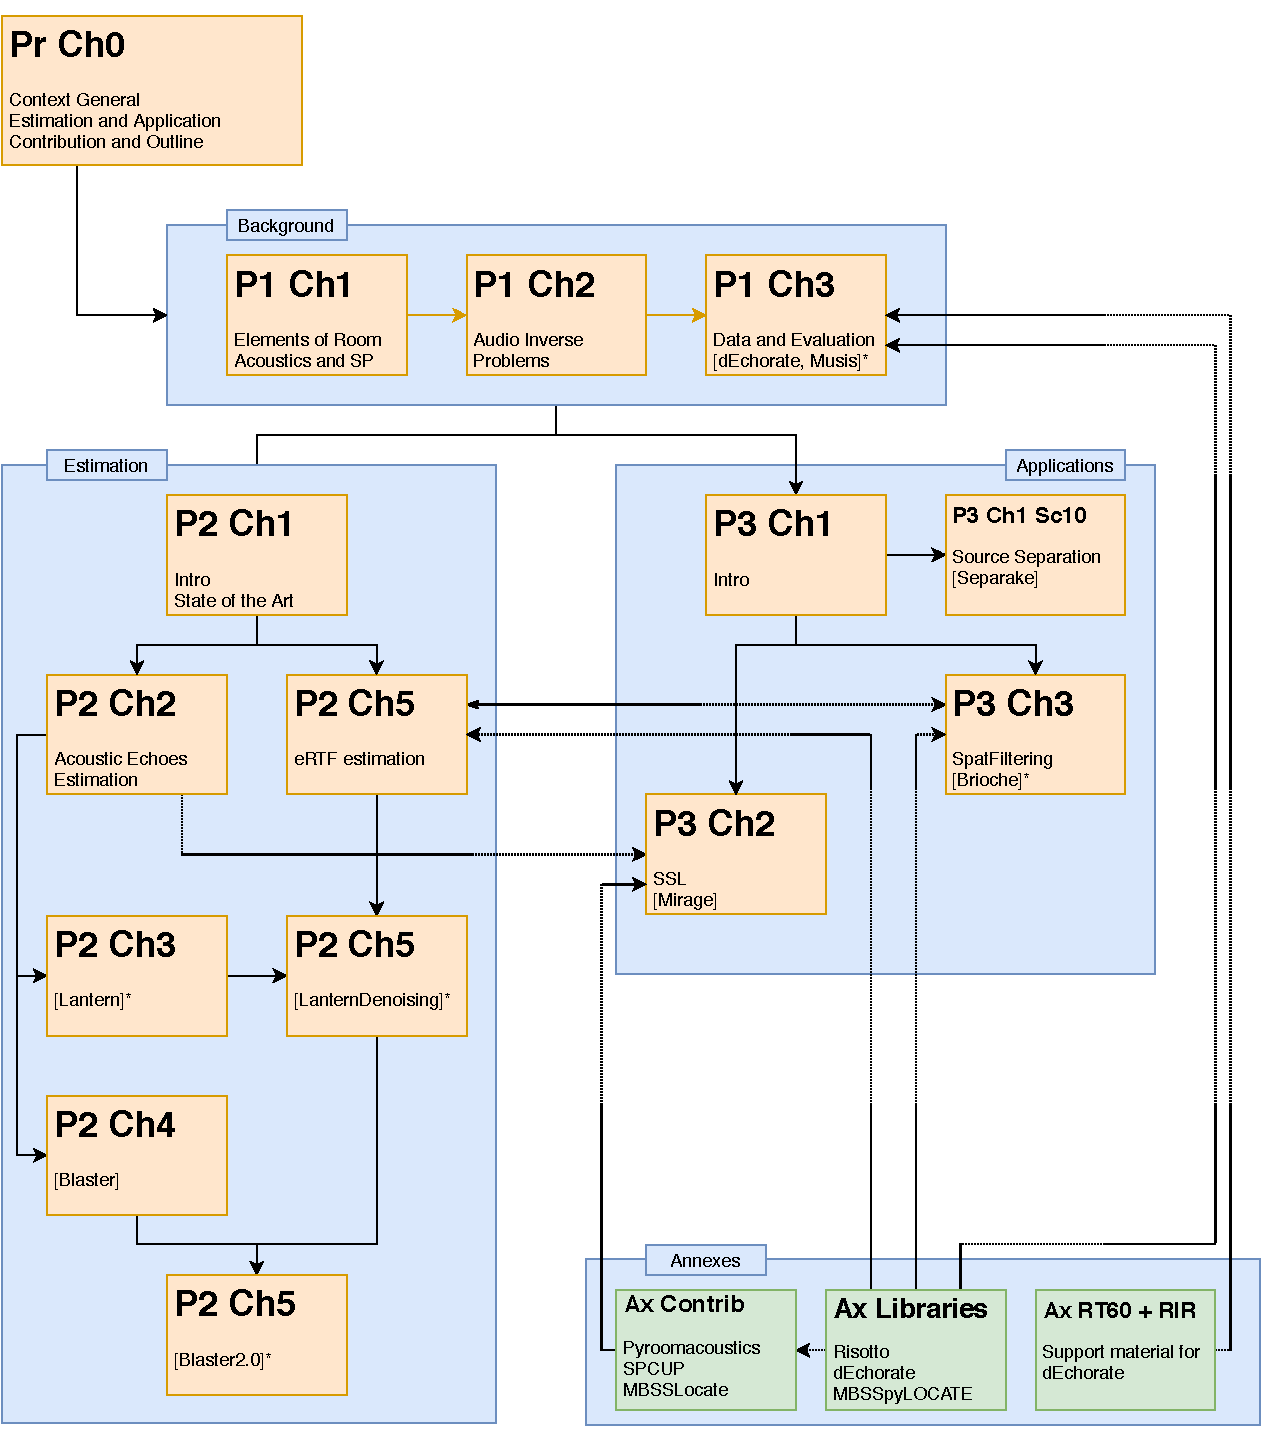
\includegraphics[width=\linewidth]{contents/assets/mindmaps/thesis_mindmap.pdf}
        \end{sidecaption}
\end{figure}


\section{Todos and Notes}

\itodo{Can we use \bison/'s argument (regarding differential cryptanalysis) for a maximal unbalanced Feistel network?}
\miss{Here something is missing}
\todo[inline]{The original todo note withouth changed colours.\newline Here's another line.}

\lipsum[11]\unsure{Is this correct?}\unsure{I'm unsure about also!}
\lipsum[11]\change{Change this!}
\lipsum[11]\info{This can help me in chapter seven!}
\lipsum[11]\plus{What was I thinking?!}
\lipsum[11]
\plus[inline]{The following section needs to be rewritten!}
\lipsum[11]

% \newthoughtpar{Incentives for new Cipher Designs}
% \blindtext

% \section{Section 1}
% \blindtext[3]

% \marginpar{%
%     \footnotesize
%     \vspace{\baselineskip}
%     \vspace*{-7\baselineskip}
%     See \cref{ch:intro} for a detailed explanation of differential cryptanalysis
%     and the problems that appear when trying to bound the differential probability.
% }

% \begin{problem}[Differentials]\label{prob:differentials}
%     \blindtext
% \end{problem}



% \section{Publications}

% During the course of my doctoral studies, I worked on several projects which are not all covered in the remainder of this thesis.
% In particular, these are the following.

% \newthoughtpar{Conference Publications}
% \begin{itemize}
% \item[] \fullfullcite{EC:CLLNW19}, see \cref{ch:bison}.
% %Because \bison/ can only be instantiated with odd block length, we here also give a second instance of the underlying construction: \wisent/.
% %This instance is for the even block length case and basically inherits almost the same security bounds as \bison/.
% \end{itemize}

% \newthoughtpar{Journal Publications}
% \begin{itemize}
%     \item[] \fullfullcite{ToSC:KraLeaWie17}.
%     \item[] \fullfullcite{ToSC:KLSW17}, see \cref{ch:slp}.
%     \item[] \fullfullcite{ToSC:LeaTezWie18}, see \cref{ch:st}.
% \end{itemize}


% \section{Stir of Echoes}

% \blindtext

% \section{Equations}

\begin{align}
    f(x) &= x^2\\
    g(x) &= \frac{1}{x}\\
    F(x) &= \int^a_b \frac{1}{3}x^3
\end{align}


A simple equation:
\[
 f(x)=(x+a)(x+b)
\]
An equation with text:
\begin{equation}
50 \text{ apples} \times 100 \text{ apples} =
\textbf{lots of apples}
\end{equation}
One including subscripts and superscripts:
\[ k_{n+1} = n^2 + k_n^2 - k_{n-1} \]
\section{Greek Letters}
\[ \alpha,  \beta,  \gamma, \Gamma, \pi, \Pi, \phi, \varphi, \mu, \Phi, \xi, \zeta \]
\[ \cos(2\theta\phi) = \cos^2 \theta\phi - \sin^2 \theta\phi \]
\section{Delimiters}
There are many types of delimiters one can use:
\[ ( a ), [ b ], \{ c \}, | d |, \| e \|,
\langle f \rangle, \lfloor g \rfloor,
\lceil h \rceil, \ulcorner i \urcorner \]
See how the delimiters are of reasonable size in these examples
\[
        \left(a+b\right)\left[1-\frac{b}{a+b}\right]=a\,,
\]
\[
        \sqrt{|xy|}\leq\left|\frac{x+y}{2}\right|,
\]
even when there is no matching delimiter
\[
        \int_a^bu\frac{d^2v}{dx^2}\,dx
        =\left.u\frac{dv}{dx}\right|_a^b
        -\int_a^b\frac{du}{dx}\frac{dv}{dx}\,dx.
\]
whereas vector problems often lead to statements such as
\[
        u=\frac{-y}{x^2+y^2}\,,\quad
        v=\frac{x}{x^2+y^2}\,,\quad\text{and}\quad
        w=0\,.
\]
\section{Multiple Fractions}
Typesetting continued fractions is easy:
\[
x = a_0 + \frac{1}{a_1 + \frac{1}{a_2 + \frac{1}{a_3 + a_4}}}
\]
However, as the fractions continue, they get smaller. If you want to keep the size consistent, use the display style; e.g.
\[
  x = a_0 + \frac{1}{\displaystyle a_1
          + \frac{1}{\displaystyle a_2
          + \frac{1}{\displaystyle a_3 + a_4}}}
\]
\section{Arrays}
Arrays of mathematics are typeset using one of the matrix environments as
in
\[
        \begin{bmatrix}
                1 & x & 0 \\
                0 & 1 & -1
        \end{bmatrix}\begin{bmatrix}
                1  \\
                y  \\
                1
        \end{bmatrix}
        =\begin{bmatrix}
                1+xy  \\
                y-1
        \end{bmatrix}.
\]
\[ \begin{pmatrix}
2 & 3 & 4\\
5 & 6 & 7\\
8 & 9 & 10 \end{pmatrix} v = 0 \]
Case statements use cases:
\[
        |x|=\begin{cases}
                x, & \text{if }x\geq 0\,,  \\
                -x, & \text{if }x< 0\,.
        \end{cases}
\]
Many arrays have lots of dots all over the place as in
\[
        \begin{matrix}
                -2 & 1 & 0 & 0 & \cdots & 0  \\
                1 & -2 & 1 & 0 & \cdots & 0  \\
                0 & 1 & -2 & 1 & \cdots & 0  \\
                0 & 0 & 1 & -2 & \ddots & \vdots \\
                \vdots & \vdots & \vdots & \ddots & \ddots & 1  \\
                0 & 0 & 0 & \cdots & 1 & -2
        \end{matrix}
\]
\section{Greek Letters}
\[ \alpha,  \beta,  \gamma, \Gamma, \pi, \Pi, \phi, \varphi, \mu, \Phi, \xi, \zeta \]
\[ \cos(2\theta\phi) = \cos^2 \theta\phi - \sin^2 \theta\phi \]
\section{Delimiters}
\[ ( a ), [ b ], \{ c \}, | d |, \| e \|,
\langle f \rangle, \lfloor g \rfloor,
\lceil h \rceil, \ulcorner i \urcorner \]
\section{Accents}
Mathematical accents are performed by a short command with one
argument, such as
\[
        \tilde f(\omega)=\frac{1}{2\pi}
        \int_{-\infty}^\infty f(x)e^{-i\omega x}\,dx\,,
\]
or
\[
        \dot{\vec \omega}=\vec r\times\vec I\,.
\]
\section{Multiline equations and aligned environments}
New lines (\\ ) do not work in equation environments. To achieve alignment of equations, use the aligned  package to produce multiline aligned math, such as:
\newline

% \[
% \begin{center}
% \begin{aligned}
% $F$ ={} & $\{F_{x} \in  F_{c} : (|S| > |C|)$ \\
%       & $\cap (\mathrm{minPixels}  < |S| < \mathrm{maxPixels})$ \\
%       & $\cap (|S_{\mathrm{conected}}| > |S| - \epsilon) $\}
% \end{aligned}
% \end{center}
% \]

% \newline

% and also:

% \newline
% \[
% \begin{center}
% \begin{aligned}
% $A_0$ & $=   \frac{1}{(\alpha+t_x)^{r+s+x}}{}_2 F_1\left( r+s+x,x+1;r+s+x+1;\frac{\alpha-\beta}{\alpha + t_x} \right) $\\
% & $\quad - \frac{1}{(\alpha+T)^{r+s+x}}{}_2 F_1\left( r+s+x,x+1;r+s+x+1;\frac{\alpha-\beta}{\alpha + T} \right),$
% \end{aligned}
% \end{center}
% \]
% \newline

\textbf{Note}: the above multiline equations have math mode defined per line, not globally at the equation level.
\section{Theorems and sets}

% \newtheorem{theorem}{Theorem}
% \newtheorem{corollary}[theorem]{Corollary}
% \newtheorem{lemma}[theorem]{Lemma}
% \newtheorem{definition}[theorem]{Definition}

\begin{theorem}
For any nonnegative integer $n$, we have
$$(1+x)^n = \sum_{i=0}^n {n \choose i} x^i$$
\end{theorem}
The Taylor series expansion for the function $e^x$ is given by
\begin{equation}
e^x = 1 + x + \frac{x^2}{2} + \frac{x^3}{6} + \cdots = \sum_{n\geq 0} \frac{x^n}{n!}
\end{equation}
\[ \forall x \in X, \quad \exists y \leq \epsilon \]
\[ \frac{n!}{k!(n-k)!} = \binom{n}{k} \]
\begin{theorem}
For any sets $A$, $B$ and $C$, we have
$$ (A\cup B)-(C-A) = A \cup (B-C)$$
\end{theorem}

\blindtext
\blinditemize

\blindtext
\blindenumerate

\blindtext
\blinddescription

\begin{fullwidth}
    \part{conclusion}
\end{fullwidth}
\chapter{Lorem}\label{chap:lorem}

\blindtext[10]

\begin{fullwidth}
    \part{Epilogue}
\end{fullwidth}
\chapter{Conclusion}\label{ch:conclusion}
\openepigraph{But at the laste, every thing hath ende}{Geoffrey Chaucer}
Since the development of the \DES/ and \AES/, our understanding of secure designs for encryption schemes has greatly evolved.
In particular in the area of symmetric cryptography, we are today, after more than 40 years of research, able to design very efficient ciphers, which we firmly believe to be secure -- with the \AES/ being the prime example withstanding 20 years of cryptanalysis.
Our progress pushed efficiency bounds further and further, especially within the trend of lightweight cryptography.

However the time may has come where we should shift our focus to improving security arguments for new designs -- because the improvement since the development of bounds for differential and linear cryptanalysis seems marginal.
We see this thesis, specifically the first part on security arguments, as a step in this direction.
With our block cipher instances \bison/ and \wisent/ we are for the first time able to give precise bounds on the \emph{differential} instead of only on differential trails.
This initial result may lead to further investigation of alternative constructions for block ciphers.
An interesting question in this direction is if a construction can be found which exhibits similar good properties with respect to linear cryptanalysis.
A second worthwhile direction is the study of unbalanced Feistel networks which seem to be related to the \WSN/ construction.

Apart from our results on differential cryptanalysis, our study of the \ACT/ revealed a connection between differential-linear cryptanalysis and previously studied properties of Boolean functions.
In our opinion the most interesting observation, from a cryptanalytic perspective, is that the decryption function might be weaker than the encryption against differential-linear attacks.
This result implies future analysis has to be extended in this direction.
From a more theoretical point of view, it is interesting that vectorial Boolean functions exhibit a lower bound for the absolute indicator, while for Boolean functions it seems to be a hard problem finding such a lower bound.
Overall, our results on this new connection contribute to a further understanding of differential-linear cryptanalysis.

In the second part of the thesis, we concentrated on automated tools for the design and analysis of block ciphers.
Our main result here was the conceptual simple algorithm for propagating subspaces through an iterative round function.
Despite the underlying simple idea, this algorithm turns out to be useful not only for one application.
For its original purpose, we use \textsc{Compute Trail} to algorithmically bound the longest subspace trail through an \SPN/ cipher and thus construct an algorithmic security argument against this recent type of attack.

However, besides the study of single attacks, a more principle task is to extend a distinguishing attack into a key recovery.
Especially when such an extension is possible over some rounds, it might make the difference between a cipher with a thin security margin and a broken one.
Thus, while being a very important part of cryptanalysis, finding key recovery strategies remains a highly manual, and thus error prone, task.
As discussed in the last chapter, our subspace trail algorithm may be used in an automatisation approach for exactly this problem -- albeit working out the exact techniques for such an automated key recovery remains to be done.

Apart from these possibilities for automated tools discussed in this thesis, a different application are cryptanalysis techniques based on \MILPp/.
We only briefly mentioned \MILPp/ for bounding the number of active S-boxes.
However, they have by now a broad spectrum of use cases, \eg/ for finding differential or linear trails, for finding division properties or similar.
All these applications have the same basic process that needs the cipher under scrutiny and the analysis technique to be modeled as an instance of the specific programming style, \ie/ as a \MILP/.
The needed building blocks for these models are known for every typical part used in ciphers, still the cryptanalyst has to assemble the models manually.
Again this is a tedious and error prone task which could easily be automated.
The development of such a \MILP/ compiler (or similarly a SAT compiler for constrained programming models) quite likely requires techniques from programming languages and compiler theory.
It seems to be an interesting problem to work on.

Finding the best representation of a cipher for these models (both for \MILPp/ and SAT) is another problem which yet remains unsolved.
This occurs especially when modeling the nonlinear S-boxes, for which different approaches exist: broadly speaking one could model the S-box in full detail, or try to pre-optimise the model on a varying level.
Similar to the XOR count optimisations it is then unclear, how much pre-optimisation helps in the end and what level of optimisation restricts the solver too much for its own optimisation strategies.


\backmatter{}

\begin{fullwidth}
\printbibliography{}
\end{fullwidth}

\cleardoublepage{}

%%%% APPENDIX

\begin{appendices}
\chapter{Mindmaps}

\Blindtext
\end{appendices}

\end{document}
